\section{Descripci\'on general}
La herramienta LabTool ofrece la posibilidad de realizar mediciones autom\'aticamente. Sus dos funciones posibles permiten medir
el diagrama de bode o respuesta en frecuencia de un circuito, as\'i como tambi\'en la impedancia de entrada del mismo. Para esto
es necesario conectarse a un osciloscopio y a un generador.

La herramiento es capaz de identificar autom\'aticamente los dispositivos conectados, actualmente s\'olo soporta:
\begin{itemize}
    \item Osciloscopio Agilent DSO6014A
    \item Osciloscopio Agilent DSO7014A
    \item Generador de funciones Agilent 33220A
\end{itemize}

\section{Requisitos del programa}
El programa est\'a desarrollado en Python 3, no obstante independientemente de esto es necesario descargar el paquete de NiVISA
para tener soporte de la comunicaci\'on, y luego instalar s\'i instalar Python y los paquetes necesarios para este. Entre los cuales se encuentran:
\begin{itemize}
    \item PyVisa
    \item Numpy
    \item PyQt5
    \item Matplotlib
    \item Openpyxl
    \item xlwt
\end{itemize}

\section{Instalaci\'on del programa}
En t\'erminos generales, para poder descargar el programa es necesario clonar el repositorio de GitHub.

\begin{center}
    \textbf{git clone https://github.com/Kammann123/lab-tool.git}
\end{center}

Luego habiendo instalado previamente Python, se pueden descargar todos los paquetes necesarios de forma autom\'atica
ejecutando en consola el siguiente comando. Es importante mencionar que para tener disponible desde la consola el instalador de pip,
este \'ultimo debe estar en las variables de entorno del sistema para el caso de Windows.

\begin{center}
    \textbf{pip install -r requirements}
\end{center}

Finalmente, se puede ejecutar el programa corriendo con Python el archivo dentro de la carpeta "lab-tool" denominado "main.py".

\begin{center}
    \textbf{python main.py}
\end{center}

\section{Conexi\'on de dispositivos}
Al ejecutar el programa, la pantalla inicial ilutra la conexi\'on con los dispositivos. Es necesario tener conectados por USB
tanto un osciloscopio como un generador, luego apretar el bot\'on de refresh para identificarlos, as\'i finalmente se podr\'a habilitar
el bot\'on para continuar.

\begin{figure}[H]
    \centering
        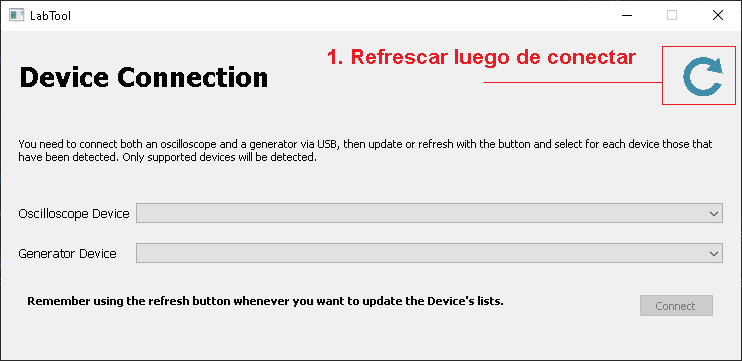
\includegraphics[scale=0.75]{../screenshots/primer_paso.png}
    \caption{Ventana inicial de conexi\'on}
\end{figure}

\begin{figure}[H]
    \centering
        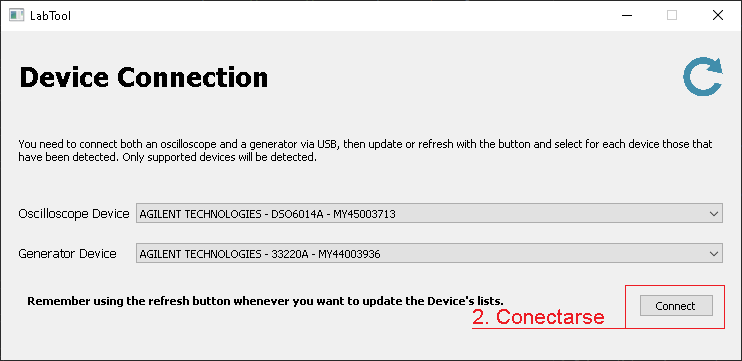
\includegraphics[scale=0.75]{../screenshots/conexion_establecido.PNG}
    \caption{Conexi\'on establecida con dispositivos}
\end{figure}

\section{Ventana del men\'u principal}
En el men\'u principal se puede seguir visualizando los dispositivos conectados. Por otro lado, en la esquina superior derecha hay tres comandos
que son para realizar acciones de configuraci\'on o desconexi\'on.
\begin{itemize}
    \item Desconectar: Desconecta los equipos y vuelve a la ventana anterior.
    \item Configurar Osciloscopio: Abre la ventana para configurar el osciloscopio.
    \item Configurar Generador: Configuraci\'on del generador y preferencias generales.
\end{itemize}

Por otro lado, en la parte de abajo est\'an los botones para configurar las mediciones y empezar a hacerlas.

\begin{figure}[H]
    \centering
        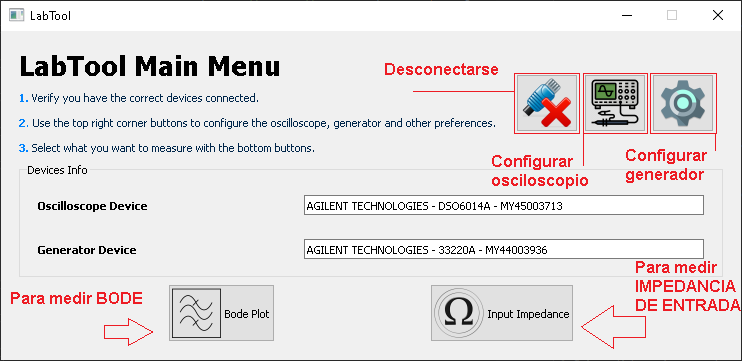
\includegraphics[scale=0.8]{../screenshots/main_menu.PNG}
    \caption{Conexi\'on y men\'u principal}
\end{figure}

\begin{figure}[H]
    \centering
    \begin{tabular}{c c}
        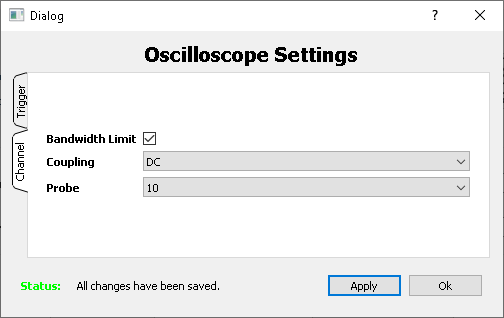
\includegraphics[scale=0.5]{../screenshots/oscilloscope_settings.PNG} &
        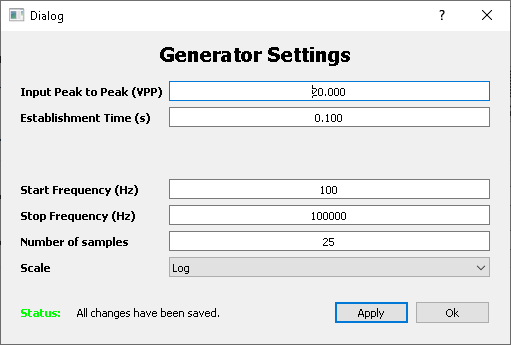
\includegraphics[scale=0.5]{../screenshots/generator_settings.PNG}
    \end{tabular}
    \caption{Ventanas de configuraci\'on}
\end{figure}

\section{Ventanas de medici\'on}
En el momento de apretar cualquiera de las dos opciones para medir, se abren dos ventanas de configuraci\'on para definir
algunos de los par\'ametros que son necesarios para ello. En el caso de la respuesta en frecuencia del circuito, es necesario definir
el canal de entrada y el de salida. Mientras que para la impedancia de entrada, es necesario adem\'as indicar qu\'e valor auxiliar se emplea.

\begin{figure}[H]
    \centering
        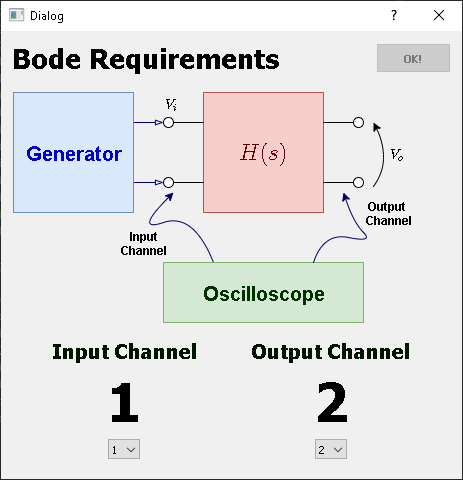
\includegraphics[scale=0.9]{../screenshots/bode_run.PNG}
    \caption{Configuraci\'on de la medici\'on de Bode}
\end{figure}

\begin{figure}[H]
    \centering
        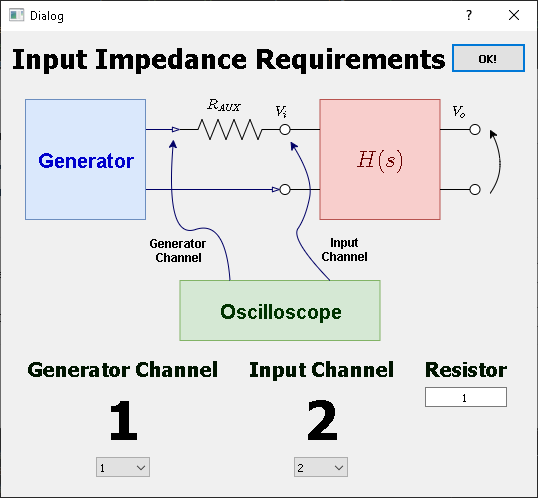
\includegraphics[scale=0.9]{../screenshots/impedance_run.PNG}
    \caption{Configuraci\'on de la medici\'on de $Z_i$}
\end{figure}

\section{Ventana del proceso de la medici\'on}
Una vez que se configuran todos los aspectos necesarios para realizar la medici\'on,
luego aparece una nueva ventana para administrar el proceso de las mediciones.
En este \'ultimo se puede dar inicio, parar o reiniciar directamente las mediciones.
Adem\'as, luego de terminar tales mediciones, se las puede visualizar gr\'aficamente o exportar en un excel.

\begin{figure}[H]
    \centering
        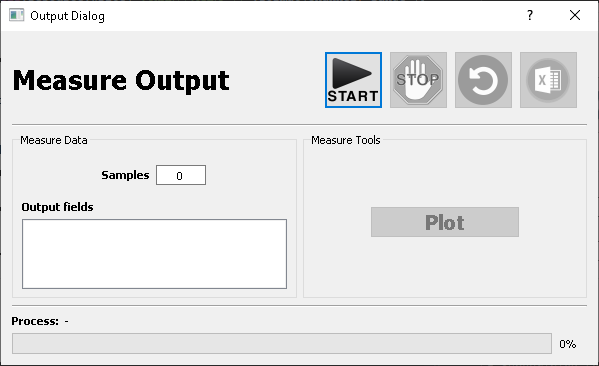
\includegraphics[scale=0.8]{../screenshots/output_screen.PNG}
    \caption{Ventana de mediciones}
\end{figure}

\begin{figure}[H]
    \centering
        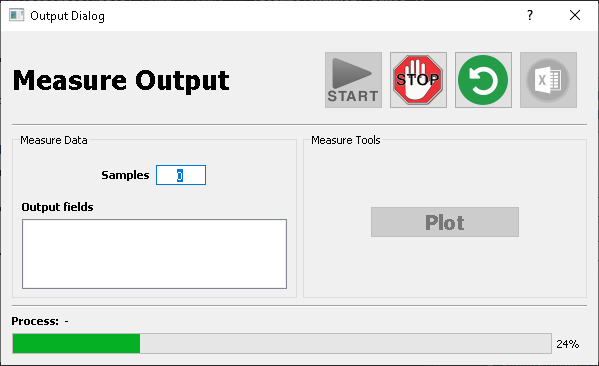
\includegraphics[scale=0.8]{../screenshots/measuring_output.PNG}
    \caption{Ventana de mediciones}
\end{figure}

\begin{figure}[H]
    \centering
        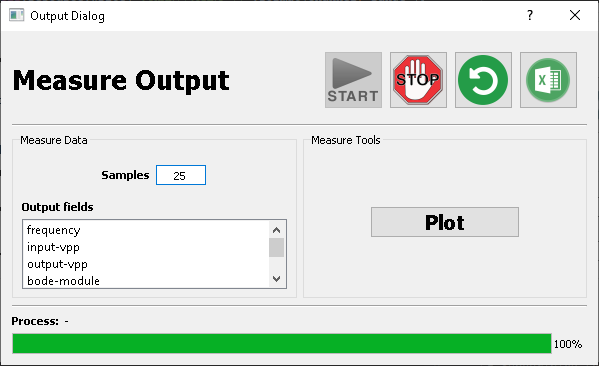
\includegraphics[scale=0.8]{../screenshots/measure_complete.PNG}
    \caption{Ventana de mediciones}
\end{figure}

\begin{figure}[H]
    \centering
        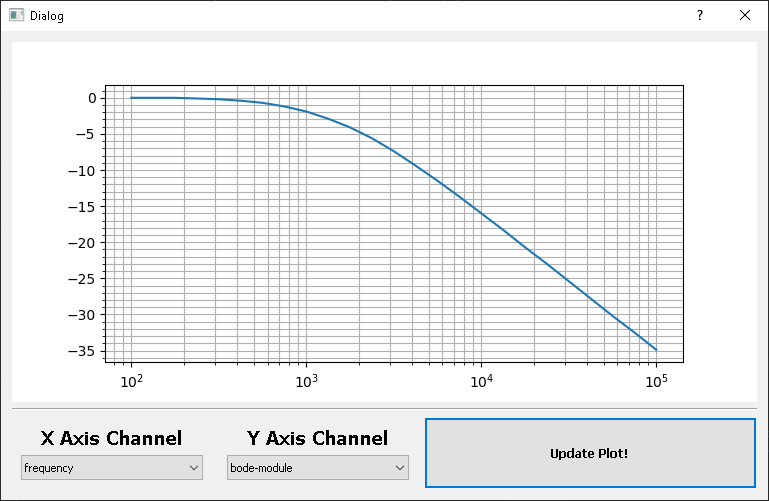
\includegraphics[scale=0.6]{../screenshots/plotter_output.PNG}
    \caption{Ventana de mediciones}
\end{figure}
